%%\begin{document}
\begin{center}
    {\it{
 by Marcela Carena, Zhen Liu, and Marc Riembau}}
 \end{center}


The singlet SM extension  serves as the simplest, yet elusive benchmark to test  a sufficiently strong  first-order phase transition (EWPT) compatible with the Higgs boson mass measurements at the LHC.
The singlet without $Z_2$ protection could mix with the SM Higgs and (in most cases) a promptly decaying scalar particle would provide a rich phenomenology at colliders. The singlet scalar could be produced resonantly  and decay back to pairs of SM particles, dominantly into $WW$, $ZZ$, $HH$ and $t\bar t$. The signal of  a singlet scalar resonance decaying into $HH$ is a smoking-gun  for singlet enhanced EWPT~\cite{Profumo:2007wc,Chen:2014ask,Dawson:2015haa,Kotwal:2016tex,Chen:2017qcz,Huang:2017jws,Robens:2016xkb,Lewis:2017dme,Dawson:2016ugw,Huang:2017nnw,deFlorian:2016spz} (see also the discussion in Section 3.6.2). 


Searches for resonant di-Higgs production have received much attention by both the ATLAS and CMS collaborations~\cite{Aaboud:2016xco,Aad:2015xja,Sirunyan:2017djm,CMS-PAS-HIG-17-006,CMS-PAS-HIG-17-008,CMS-PAS-HIG-17-009}. In the case of a singlet resonance,  constraints from SM precision measurements  render these searches more challenging. From one side  precision measurements  imply that  the singlet-doublet mixing parameter is constrained to be small over a large region of parameter space.  On the other side, the singlet only couples to SM particles through mixing with the SM Higgs doublet. This results in a reduced di-Higgs production via singlet resonance decays. In particular, the singlet resonance amplitude  becomes of the same order as the SM  triangle  and box diagram amplitudes. Most important, in this work we shall show that a large relative phase between the SM box diagram and the singlet triangle diagram becomes important. This special on-shell interference  effect  has been  commonly overlooked in the literature and turns out to have important phenomenological implications.
We shall choose the spontaneous $Z_2$ breaking scenario of the SM plus singlet to demonstrate the importance of the novel on-shell interference effect for the resonant singlet scalar searches in the di-Higgs production mode.

\subsubsubsection{Model framework}
\label{sec:model}

We will consider the simplest extension of the SM that can assist the scalar potential to induce a strongly first-order electroweak phase transition, consisting of an additional real scalar singlet with a $Z_2$ symmetry. The scalar potential of the model can be written as
\be
V(s,\phi)=-\mu^2 \phi^\dagger \phi -\frac 1 2 \mu_s^2 s^2 +  \lambda (\phi^\dagger \phi)^2 + \frac {\lambda_s} {4} s^4 + \frac {\lambda_{s\phi}} 2 s^2 \phi^\dagger\phi,
\label{eq:potential}
\ee
where $\phi$ is the SM doublet
\footnote{ $\phi^T=(G^+,\frac 1 {\sqrt{2}} (h+ i G^0 +v))$, where $G^{\pm,0}$ are the Goldstone modes.}
and $s$ represents the new real singlet field. In the above, we adopt the conventional normalization for the couplings of the SM doublets and match the other couplings with the singlet with identical normalization. We allow for spontaneous $Z_2$ breaking with the singlet $s$ acquiring a vacuum expectation value $v_s$, since this case allows for interesting collider phenomenology of interference effects. As we shall show  later, the (on-shell) interference effects commonly exist for  loop-induced processes in BSM phenomenology and it is the focus of this paper. The CP even neutral component $h$ of the Higgs doublet field $\phi$ mixes with the real singlet scalar $s$, defining the new mass eigenstates $H$ and $S$
\bea
\binom{h}{s} =  \begin{pmatrix}
 \cos\theta & \sin\theta \\
 -\sin\theta & \cos\theta 
 \end{pmatrix}
 \binom{H}{S},
\eea
where $\theta$ is the mixing angle between these fields.
% and $h$ does not include the Higgs vev of $v$. 
%The capitalized $H$ and $S$ represent mass eigenstates that are mostly from the SM doublet $\phi$ and mostly singlet $s$, respectively. 
The five free parameters in Eq.~(\ref{eq:potential}) can  be traded by the two boundary conditions 
\be
m_{H}= 125~\UGeV,~~v=246~\UGeV
\ee
and the three ``physical'' parameters,
\be
m_S,~~\tan\beta(\equiv \frac  {v_s} v),~{\rm and~}\sin\theta,\label{eq:basis}
\ee
where $\tan\beta$ characterizes the ratio between the vevs of the doublet and the singlet scalar fields, respectively. Detailed relations between the bare parameters and physical parameters can be found in Ref.~\cite{Carena:2018vpt}.

\subsubsubsection{Enhancing the di-Higgs signal via interference effects}
\label{sec:interference}


The on-shell interference effect may enhance or suppress the conventional Breit-Wigner resonance production. 
Examples in Higgs physics known in the literature, such as $gg\to h\to\gamma\gamma$~\cite{Campbell:2017rke} and $gg\to H\to t\bar t$~\cite{Dicus:1994bm,Carena:2016npr,Gori:2016zto,Craig:2015jba,Jung:2015gta}, are both destructive.
We discuss in detail in this section the on-shell interference effect between the resonant singlet amplitude and the SM di-Higgs box diagram. We shall show that in the singlet extension of the SM considered in this paper, the on-shell interference effect is generically constructive and could be large in magnitude, thus enhances the signal production rate. 


The interference effect between two generic amplitudes can be denoted as nonresonant amplitude $A_{nr}$ and resonant amplitude $A_{res}$.
The resonant amplitude $A_{res}$, defined as
\be
A_{res} = a_{res} \frac {\hat s} {\hat s - m^2 + i \Gamma m},
\ee
has a pole in the region of interest and 
we parametrize it as the product of a fast varying piece containing its propagator and a slowly varying piece $a_{res}$ that generically is a product of couplings and loop-functions. The general interference effect can then be parametrized as~\cite{Carena:2016npr,Campbell:2017rke},
\bea
|\mathcal{M}|_{int}^2 &=& 2\Re(A_{res}\times A_{nr}^*)\,=\,2\left(\mathcal{I}_{int} + \mathcal{R}_{int}\right),\nonumber \\
\mathcal{R}_{int} &\equiv& |A_{nr}||a_{res}|\frac {\hat s (\hat s - m^2)} {(\hat s - m^2)^2+\Gamma^2 m^2} \cos(\delta_{res}-\delta_{nr})\nonumber \\
\mathcal{I}_{int} &\equiv& |A_{nr}||a_{res}|\frac {\hat s \Gamma m} {(\hat s - m^2)^2+\Gamma^2 m^2} \sin(\delta_{res}-\delta_{nr}),
\label{eq:decomposition}
\eea
where $\delta_{res}$ and $\delta_{nr}$ denote the complex phases of $a_{res}$ and $A_{nr}$, respectively.

The special interference effect $\mathcal{I}_{int}$ only appears between the singlet resonant diagram and the SM box diagram. This interference effect is proportional to the relative phase between the loop functions $\sin(\delta_\vartriangleright-\delta_\square)$ and the imaginary part of the scalar propagator which is sizable near the scalar mass pole. 


\subsubsubsection{Differential distribution}

\begin{figure}[t]  
  \centering
  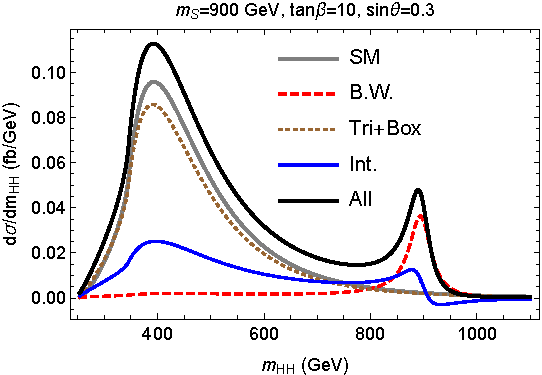
\includegraphics[width=.60\textwidth]{\main/section9/plots/linearlineshape}
  %\includegraphics[width=.48\textwidth]{figs/decomposition900}
  \caption{
  The differential di-Higgs distribution for a benchmark point of the singlet extension of the SM shown in linear scale and over a broad range of the di-Higgs invariant mass. The full results for the SM and the singlet SM extension  are shown by the  gray and black curves, respectively. In the singlet extension of the SM, the contributions from the resonant singlet diagram, the nonresonant diagram and the interference between them are shown in red (dashed), brown (dotted) and blue curves, respectively.  
  %Decomposition of the differential distribution of the Higgs pair production in presences of a singlet resonance. The black curve represent the overall lineshape after coherent sum of all amplitudes squared. The red curve represent the Breit-Wigner resonance piece from the singlet resonant production. The dark blue (thick) curve represent the novel interference term between the singlet resonant amplitude and the SM box amplitude that enhances the signal resonant production, noting the identical lineshape of this contribution to that of the Breit-Wigner piece in red curves. The blue, brown and magenta lines represent the conventional interference terms $\mathcal{R}_{int}$ between the three amplitudes. We show the corresponding destructive interference effects in dashed curves. 
  %\ZL{y-axis normalization need to be updated/corrected.}
  }
  \label{fig:phenoshape} 
\end{figure}

We present in this section our analysis of the differential distribution of the Higgs pair invariant mass to estimate the relevance of the interference effects discussed in the previous section. We choose one of the best channels, $pp\to HH \to b\bar b \gamma\gamma$, as the benchmark channel to present the details of our analysis. Furthermore, we discuss another phenomenologically relevant piece of interference in the far off-shell region of the singlet scalar. We display the discovery and exclusion reach  for both HL-LHC and HE-LHC  for various values of $\tan\beta$ in the $m_S$-$\sin\theta$ plane. 

%%Before considering a full detailed analysis of interference effects and the projected results, we would like to comment on the phenomenologically important off-shell interference effect.
%, in addition to the on-shell interference effect around the pole of the heavy scalar. 
In Fig.~\ref{fig:phenoshape} we display the differential cross section as a function of the Higgs pair invariant mass for a benchmark point with a heavy scalar mass of 900 GeV, mixing angle $\sin\theta=0.3$ and $\tan\beta=10$. 
%Instead of showing the cross section in logarithmic scale and in the vicinity of the heavy scalar mass pole as in \autoref{fig:decomposition}, we show from a more observational perspective for the cross section in linear scale and a large range of the Higgs pair invariant mass, covering the low invariant mass regime favor by parton distribution functions at hadron colliders.
The differential cross section is shown in linear scale for a broad range of di-Higgs invariant masses,  including the low invariant mass regime favored by parton distribution functions at hadron colliders.

We choose this benchmark to show well the separation of the scalar resonance peak and the threshold enhancement peak above the $t\bar t$-threshold. The SM Higgs pair invariant mass distribution is given by the  gray curve while the black curve depicts the di-Higgs invariant mass distribution from the singlet extension of the SM. 
It is informative to present all three pieces that contribute to the full result of the di-Higgs production, namely, the resonance contribution (red, dashed curve), the SM nonresonance contribution (box and triangle diagrams given by the brown, dotted curve), and the interference between them (blue curve). 
Note that the small difference between the ``Tri+Box'' and the ``SM'' line shapes is caused by the doublet-singlet scalar mixing, which leads to a $\cos\theta$ suppression of the SM-like Higgs coupling to top quarks as well as a modified SM-like Higgs trilinear coupling $\lambda_{HHH}$.
We observe that the full results show an important enhancement in the di-Higgs production across a  large range of invariant masses. This behavior is anticipated from the decomposition analysis in the previous section. There is a clear net effect from  the interference curve shown in blue.  Close to the the scalar mass pole at 900 GeV, the on-shell interference effect enhances the Breit-Wigner resonances peak (red, dashed curve) by about 25\%. Off-the resonance peak, and especially at the threshold peak, the interference term (blue curve) enhances the cross section quite sizably as well. Hence, a combined differential analysis in the Higgs pair invariant mass is crucial in probing the singlet extension of the SM. 
%Moreover, a consistent treatment is required not only for the purpose of exclusion but also in extraction of the physics information contained in potential deviations. 


\subsubsubsection{Discovery and exclusion reach at the HL- and HE-LHC} 

\begin{figure}[t]
  \centering
  %\includegraphics[width=.48\textwidth]{figs/projectionHL1}
  %\includegraphics[width=.48\textwidth]{figs/projectionHE1} 
  %\includegraphics[width=.48\textwidth]{figs/projectionHL2}
  %\includegraphics[width=.48\textwidth]{figs/projectionHL10}
  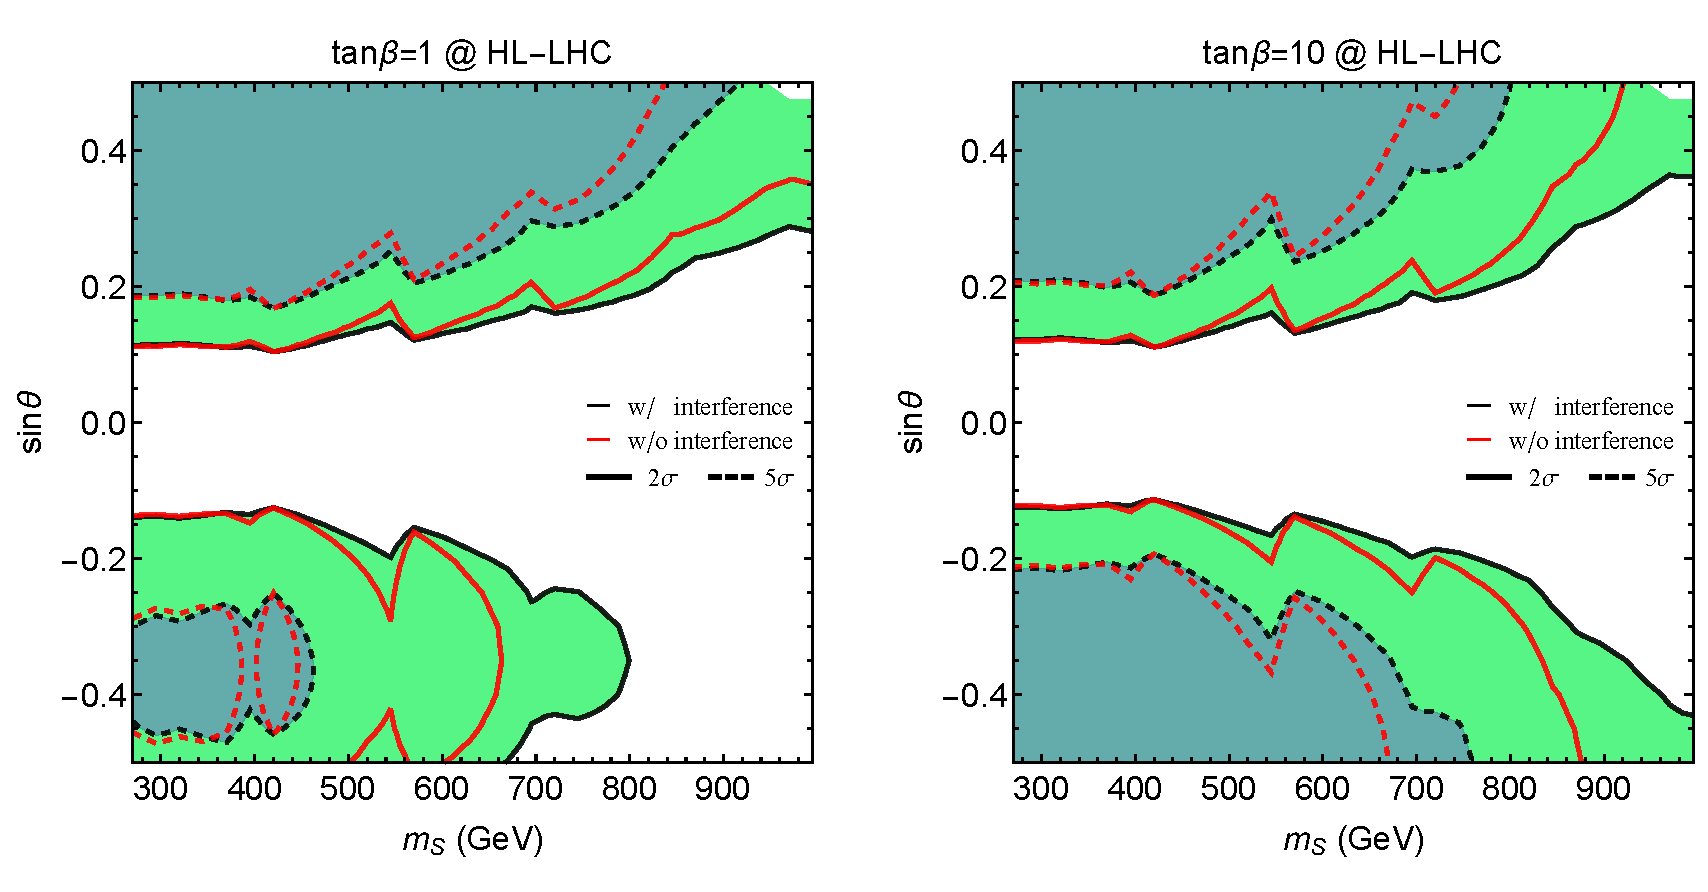
\includegraphics[width=1\textwidth]{\main/section9/plots/hllhc_projections.pdf}
  \caption{Projected exclusion and discovery limits at HL-LHC in the $m_S$-$\sin\theta$ plane with the line-shape analysis detailed in the text for $\tan\beta=1$ (left panel) and $\tan\beta=10$ (right panel). The shaded regions bounded by dashed/solid curves are within the discovery/exclusion reach of the HL-LHC. The black and red lines represent the projection with and without the inclusion of the interference effects between the singlet resonance diagram and the SM Higgs pair diagram, respectively.
  %The left, middle and right panel corresponds to $\tan\beta$ values of 1, 2 and 10 respectively. The shaded region are disallowed by vacuum stability and perturbative unitarity argument.
  }
  \label{fig:HLprojection}
\end{figure} 

Using the analysis detailed in Ref.~\cite{Carena:2018vpt} through the $pp\to HH \to \gamma\gamma b\bar b$ channel, we obtain the discovery and exclusion projections for the HL-LHC and HE-LHC.
In Fig.~\ref{fig:HLprojection} we show the projected 2-$\sigma$ exclusion and 5-$\sigma$ discovery reach for the HL-LHC in the $m_S$-$\sin\theta$ plane for $\tan\beta=1$ (left panel) and $\tan\beta=10$ (right panel) in solid and dashed curves, respectively. The shaded regions are within the reach of the HL-LHC for discovery and exclusion projections. To demonstrate the relevance of the interference effects discussed in the previous sections, we show both the results obtained with and without the inclusion of the interference effects in black and red contours, respectively. 
%We further overlay the disallowed regions from perturbative unitarity requirement and the EWPO constraints in gray and brown shaded regions, respectively.

We observe in Fig.~\ref{fig:HLprojection} that the inclusion of the interference effects extend the projections in a relevant way. For example, considering the $\tan\beta=10$ case in the right panel for $\sin\theta\simeq 0.35$ the interference effect increase the exclusion limit on $m_S$ from 850~GeV to 1000~GeV.
%, due to the large on-shell interference effects shown in the right panel of \autoref{fig:interference_central}. 
%Note that the perturbative unitarity does not constrain the parameter space of heavy scalar mass $m_S$ below a few TeV, the inclusion of the interference effect increases the discover and exclusion limit further in the sizable $\sin\theta$ region.
Note that the on-shell interference effect is larger for heavier scalar mass $m_S$. 
%, which in the cases of large $\tan\beta$ are still compatible with the perturbative unitarity requirement. 

\begin{figure}[t]
  \centering
  %\includegraphics[width=.48\textwidth]{figs/projectionHE2} 
  %\includegraphics[width=.48\textwidth]{figs/projectionHE1}
  %\includegraphics[width=.48\textwidth]{figs/projectionHL2}
  %\includegraphics[width=.48\textwidth]{figs/projectionHE10}
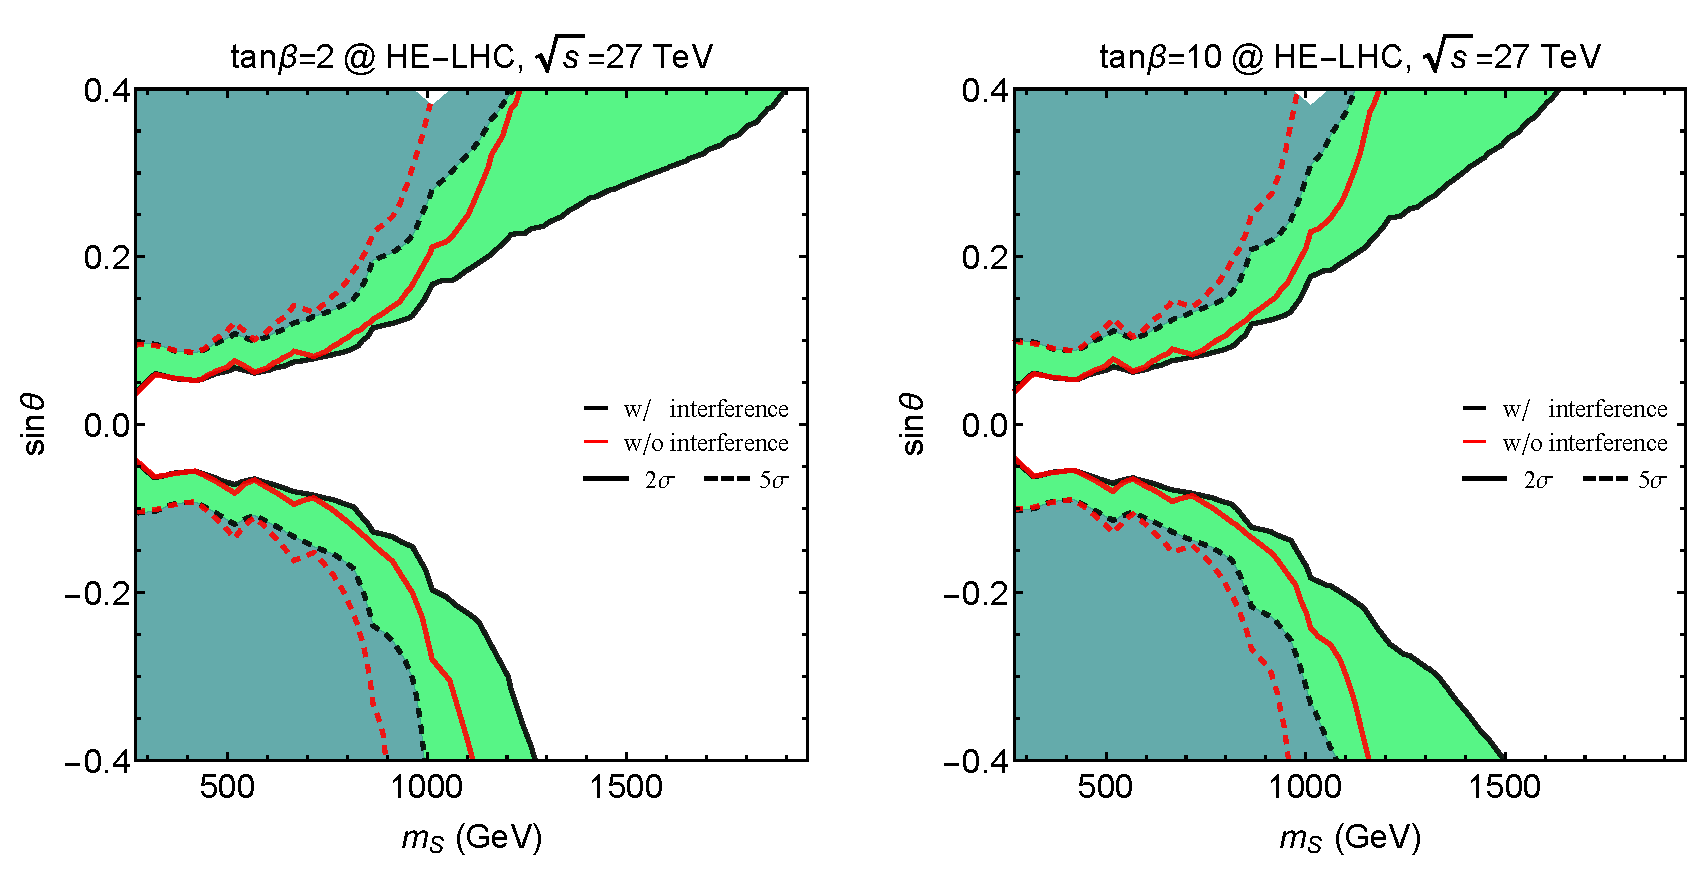
\includegraphics[width=1\textwidth]{\main/section9/plots/helhc_projections.pdf}
  \caption{
    %\ZL{figure to be updated upon new data. }
  Similar to Fig.~\ref{fig:HLprojection}, projected exclusion and discovery limits at HE-LHC with 27 TeV center of mass energy and an integrated luminosity of 10~$\abi$ for $\tan\beta=2$ (left panel) and $\tan\beta=10$ (right panel).
  %The left, middle and right panel corresponds to $\tan\beta$ values of 1, 2 and 10 respectively. The shaded region are disallowed by vacuum stability and perturbative unitarity argument.
  }
  \label{fig:HEprojection}
\end{figure} 

In Fig.~\ref{fig:HEprojection} we show the projections for the HE-LHC in a analogous fashion as in Fig.~\ref{fig:HLprojection}. The discovery and exclusion reach for heavy scalars can be significantly extended by the HE-LHC operating at 27 TeV center of mass energy with 10 $\abi$ of integrated luminosity. We show the results for $\tan\beta=2$ (left panel) and $\tan\beta=10$ (right panel). 
For example, considering the $\tan\beta=2$ case in the right panel of Fig.~\ref{fig:HEprojection}, for $\sin\theta\simeq 0.35$ the exclusion reach increases from 1200 to 1800~GeV, once more showing the importance of including the on-shell interference effects.

\subsubsubsection{Summary and outlook}
\label{sec:conclude}

In this study, we analyze the interference effects in the $gg\to HH$ process in the presence of a heavy scalar resonance.
We focus on the novel effect of the on-shell interference contribution and discuss it in detail considering the framework of the singlet extension of the SM with spontaneous $Z_2$ breaking. % in the singlet sector.
The interference pattern between the resonant heavy scalar contribution and the SM nonresonant triangle and box contributions show interesting features. 
%A detailed decomposition of the interference pattern is presented in \autoref{sec:interference} and 
We highlight the constructive on-shell interference effect that uniquely arises between the heavy scalar resonance diagram and the SM box diagram, due to a large relative phase between the loop functions involved.
% shown in \autoref{fig:phase}. 
%We further quantify the size of this constructive on-shell interference effect by showing its strength in \autoref{fig:interference_central}. 
We observe that the on-shell interference effect can be as large as 40\% of the Breit-Wigner resonance contribution and enhances notably the total signal strength, making it necessary taking into account in heavy singlet searches.

To better evaluate the phenomenological implications of the interference effects in the di-Higgs searches, we carried out a line-shape analysis in the $gg\to HH \to \gamma\gamma b\bar b$ channel, taking into account both the on-shell and off-shell interference contributions. We find that both for the HL-LHC and HE-LHC, the proper inclusion of the interference effects increases the discovery and exclusion reach significantly.

%%\end{document}
